%%%%%%%%%%%%%%%%%%%%%%%%%%%%%%%%%%%%%%%%%
% Programming/Coding Assignment
% LaTeX Template
%
% This template has been downloaded from:
% http://www.latextemplates.com
%
% Original author:
% Ted Pavlic (http://www.tedpavlic.com)
%
% Note:
% The \lipsum[#] commands throughout this template generate dummy text
% to fill the template out. These commands should all be removed when 
% writing assignment content.
%
% This template uses a Perl script as an example snippet of code, most other
% languages are also usable. Configure them in the "CODE INCLUSION 
% CONFIGURATION" section.
%
%%%%%%%%%%%%%%%%%%%%%%%%%%%%%%%%%%%%%%%%%

%----------------------------------------------------------------------------------------
%	PACKAGES AND OTHER DOCUMENT CONFIGURATIONS
%----------------------------------------------------------------------------------------

\documentclass{article}

\usepackage{fancyhdr} % Required for custom headers
\usepackage{lastpage} % Required to determine the last page for the footer
\usepackage{extramarks} % Required for headers and footers
\usepackage[usenames,dvipsnames]{color} % Required for custom colors
\usepackage{graphicx} % Required to insert images
\usepackage{listings} % Required for insertion of code
\usepackage{courier} % Required for the courier font
\usepackage{lipsum} % Used for inserting dummy 'Lorem ipsum' text into the template
\usepackage[dutch]{babel}
\usepackage{amsmath,amssymb}
\usepackage{float}

\newtheorem{stelling}{Stelling}
\newenvironment{proof}{\paragraph{Bewijs: }}{\hfill$\square$}


% Margins
\topmargin=-0.45in
\evensidemargin=0in
\oddsidemargin=0in
\textwidth=6.5in
\textheight=9.0in
\headsep=0.25in

\linespread{1.1} % Line spacing

% Set up the header and footer
\pagestyle{fancy}
\lhead{ } % Top left header
\chead{ } % Top center head
\rhead{ } % Top right header
\lfoot{\hmwkAuthorName, \hmwkAuthorNameS} % Bottom left footer
\cfoot{} % Bottom center footer
\rfoot{Pagina\ \thepage\ van\ \protect\pageref{LastPage}} % Bottom right footer
\renewcommand\headrulewidth{0.0pt} % Size of the header rule
\renewcommand\footrulewidth{0.4pt} % Size of the footer rule

\setlength\parindent{0pt} % Removes all indentation from paragraphs

%----------------------------------------------------------------------------------------
%	CODE INCLUSION CONFIGURATION
%----------------------------------------------------------------------------------------

\definecolor{MyDarkGreen}{rgb}{0.0,0.4,0.0} % This is the color used for comments
\lstloadlanguages{Perl} % Load Perl syntax for listings, for a list of other languages supported see: ftp://ftp.tex.ac.uk/tex-archive/macros/latex/contrib/listings/listings.pdf
\lstset{language=Perl, % Use Perl in this example
        frame=single, % Single frame around code
        basicstyle=\small\ttfamily, % Use small true type font
        keywordstyle=[1]\color{Blue}\bf, % Perl functions bold and blue
        keywordstyle=[2]\color{Purple}, % Perl function arguments purple
        keywordstyle=[3]\color{Blue}\underbar, % Custom functions underlined and blue
        identifierstyle=, % Nothing special about identifiers                                         
        commentstyle=\usefont{T1}{pcr}{m}{sl}\color{MyDarkGreen}\small, % Comments small dark green courier font
        stringstyle=\color{Purple}, % Strings are purple
        showstringspaces=false, % Don't put marks in string spaces
        tabsize=5, % 5 spaces per tab
        %
        % Put standard Perl functions not included in the default language here
        morekeywords={rand},
        %
        % Put Perl function parameters here
        morekeywords=[2]{on, off, interp},
        %
        % Put user defined functions here
        morekeywords=[3]{test},
       	%
        morecomment=[l][\color{Blue}]{...}, % Line continuation (...) like blue comment
        numbers=left, % Line numbers on left
        firstnumber=1, % Line numbers start with line 1
        numberstyle=\tiny\color{Blue}, % Line numbers are blue and small
        stepnumber=5 % Line numbers go in steps of 5
}

% Creates a new command to include a perl script, the first parameter is the filename of the script (without .pl), the second parameter is the caption
\newcommand{\perlscript}[2]{
\begin{itemize}
\item[]\lstinputlisting[caption=#2,label=#1]{#1.pl}
\end{itemize}
}

%----------------------------------------------------------------------------------------
%	DOCUMENT STRUCTURE COMMANDS
%	Skip this unless you know what you're doing
%----------------------------------------------------------------------------------------

% Header and footer for when a page split occurs within a problem environment
\newcommand{\enterProblemHeader}[1]{
\nobreak\extramarks{#1}{#1 continued on next page\ldots}\nobreak
\nobreak\extramarks{#1 (continued)}{#1 continued on next page\ldots}\nobreak
}

% Header and footer for when a page split occurs between problem environments
\newcommand{\exitProblemHeader}[1]{
\nobreak\extramarks{#1 (continued)}{#1 continued on next page\ldots}\nobreak
\nobreak\extramarks{#1}{}\nobreak
}

%\setcounter{secnumdepth}{0} % Removes default section numbers
%\newcounter{homeworkProblemCounter} % Creates a counter to keep track of the number of problems

%\newcommand{\homeworkProblemName}{}
%\newenvironment{homeworkProblem}[1][Problem \arabic{homeworkProblemCounter}]{ % Makes a new environment called homeworkProblem which takes 1 argument (custom name) but the default is "Problem #"
%\stepcounter{homeworkProblemCounter} % Increase counter for number of problems
%\renewcommand{\homeworkProblemName}{#1} % Assign \homeworkProblemName the name of the problem
%\section{\homeworkProblemName} % Make a section in the document with the custom problem count
%\enterProblemHeader{\homeworkProblemName} % Header and footer within the environment
%}{
%\exitProblemHeader{\homeworkProblemName} % Header and footer after the environment
%}

\newcommand{\problemAnswer}[1]{ % Defines the problem answer command with the content as the only argument
\noindent\framebox[\columnwidth][c]{\begin{minipage}{0.98\columnwidth}#1\end{minipage}} % Makes the box around the problem answer and puts the content inside
}

%\newcommand{\homeworkSectionName}{}
%\newenvironment{homeworkSection}[1]{ % New environment for sections within homework problems, takes 1 argument - the name of the section
%\renewcommand{\homeworkSectionName}{#1} % Assign \homeworkSectionName to the name of the section from the environment argument
%\subsection{\homeworkSectionName} % Make a subsection with the custom name of the subsection
%\enterProblemHeader{\homeworkProblemName\ [\homeworkSectionName]} % Header and footer within the environment
%}{
%\enterProblemHeader{\homeworkProblemName} % Header and footer after the environment
%}

%----------------------------------------------------------------------------------------
%	NAME AND CLASS SECTION
%----------------------------------------------------------------------------------------

\newcommand{\hmwkTitle}{Practicum Numerieke Wiskunde} % Assignment title
\newcommand{\hmwkSubject}{Benadering van functies door veeltermen} % Due date
\newcommand{\hmwkClass}{COMPSCI\ 101} % Course/class
\newcommand{\hmwkClassTime}{ } % Class/lecture time
\newcommand{\hmwkClassInstructor}{ } % Teacher/lecturer
\newcommand{\hmwkAuthorName}{Sarah Crombez} % Your name
\newcommand{\hmwkAuthorNameS}{Zimcke Van de Staey}

%----------------------------------------------------------------------------------------
%	TITLE PAGE
%----------------------------------------------------------------------------------------

\title{
\vspace{2in}
\textmd{\textbf{ \hmwkTitle}}\\
\vspace{0.1in}\normalsize\vspace{0.1in} \large{\hmwkSubject}\\
%\vspace{0.1in}\large{\textit{\hmwkClassInstructor\ \hmwkClassTime}}
\vspace{3in}
}

\author{\textbf{\hmwkAuthorName}\ \\ \textbf{\hmwkAuthorNameS}\ }
\date{} % Insert date here if you want it to appear below your name

%----------------------------------------------------------------------------------------

\begin{document}

\maketitle

%----------------------------------------------------------------------------------------
%	TABLE OF CONTENTS
%----------------------------------------------------------------------------------------

%\setcounter{tocdepth}{1} % Uncomment this line if you don't want subsections listed in the ToC

\newpage
\tableofcontents
\newpage

%----------------------------------------------------------------------------------------
%	PART 0
%----------------------------------------------------------------------------------------

% To have just one problem per page, simply put a \clearpage after each problem

%\begin{homeworkProblem}
\section{Achtergrond}

De Chebyshev veeltermen van de eerst soort $T_{k}(x)$ worden gedefinieerd op basis van de volgende recursiebetrekking:
\begin{center}
$T_{0}(x)=1$\\
$T_{1}(x)=x$\\
$T_{k+1}(x)=2xT_{k}(x)-T_{k-1}(x)$
\end{center}

\begin{stelling}
Op het interval $[-1,1]$ voldoen de Chebyshev veeltermen aan volgende vergelijking:
\begin{equation}
T_{k}(x)=\cos(k\arccos(x)) \label{formule1}
\end{equation}
\end{stelling}

\problemAnswer{
\begin{proof}
We zullen deze stelling aantonen met behulp van volledige inductie.\\ \\
\vspace{0.1in}
\begin{bfseries}Basisstap:\end{bfseries}\\
voor $k=0$ geldt: $T_{0}=\cos(0*\arccos(x))=\cos(0)=1$\\
voor $k=1$ geldt: $T_{1}=\cos(\arccos(x))=x$ op het interval $[-1,1]$ want de $\arccos$-functie is enkel 	gedefinieerd op het interval $[-1,1]$.\\ \\
\vspace{0.1in}
\begin{bfseries}Inductiestap:\end{bfseries}\\
We nemen aan dat voor alle $j\leq n$ geldt: $T_{n}(x)=\cos(n\arccos(x))$. Nu moet aangetoond worden dat dit ook 	geldt voor $n+1$. Volgens de recursiebetrekking voor de Chebyshev veeltermen geldt: $T_{n+1}(x)=2xT_{n}(x)-T_{n-1}(x)$. Nu kunnen we de inductiehypothese toepassen, dit geeft: $T_{n+1}(x)=2x\cos(n\arccos(x))-\cos((n-1)\arccos(x))$. Met behulp van de som-en verschilformules voor de cosinus kunnen we dit schrijven als: $T_{n+1}=2x\cos(n\arccos(x))-\cos(n\arccos(x))\cos(\arccos(x))-\sin(n\arccos(x))\sin(\arccos(x))\\
=\cos(n\arccos(x)\cos(\arccos(x))-\sin(n\arccos(x))\sin(\arccos(x))$
Hierop kunnen we dan opnieuw de som-en verschil formules voor de cosinus op toepassen en dit geeft:
$T_{n+1}(x)=\cos((n+1)\arccos(x))$. De veronderstelling geldt dus ook voor n+1.\\ \\
\vspace{0.1in}
\begin{bfseries}Conclusie:\end{bfseries}\\
Uit de basisstap, de inductiestap en het principe van volledige inductie volgt het te bewijzen.
\end{proof}
}

\clearpage 
%Listing \ref{homework_example} shows a Perl script.
%\perlscript{homework_example}{Sample Perl Script With Highlighting}
%\end{homeworkProblem}

%----------------------------------------------------------------------------------------
%	PART 1
%----------------------------------------------------------------------------------------

%\begin{homeworkProblem}

\section{Deel 1: Drie veeltermbasissen} 

 \\  \ \\
\begin{figure}[H]
\includegraphics[width=0.50\columnwidth]{chebyshev_veeltermen}
\caption{Chebyshev veeltermen tot en met graad 5} % Example image
\end{figure}


%\end{homeworkProblem}

%----------------------------------------------------------------------------------------
%	PART 2
%----------------------------------------------------------------------------------------

\section{Deel 2: Veelterminterpolatie}


\subsection{Equidistante punten en het Runge fenomeen}
 \\  \ \\

\begin{figure}[H]
\includegraphics[width=0.60\columnwidth]{lagrange_interpolatie}
\caption{Veelterminterpolatie van de Runge functie in de Lagrange basis} % Example image
\end{figure}


Figuur 2 toont dat, bij toenemende graad, de respectievelijke veelterminterpolatie \textbf{niet vanzelfsprekend een betere benadering} van de Runge functie oplevert. We zien duidelijk dat de veeltermen aan de uiteinden van het interval [-1,1] \textbf{sterkere oscillaties} vertoont. Tussen de interpolatiepunten, zal de Lagrange interpolatie een overschatting maken van de verandering in functiewaarden. Dit gedrag wordt versterkt naarmate men meer interpolatiepunten kiest. 
\\  \\
Om dit extreme gedrag in de buurt van de randwaarden te minimaliseren, kan men er voor opteren de \textbf{interpolatiepunten anders te verspreiden} over het interval. De Chebyshev punten vormen een horizontale projectie van punten op de goniometrische cirkel en zullen daarom dichter bij elkaar liggen in de buurt van -1 en 1.  
\\ \\

\begin{figure}[H]
\includegraphics[width=0.75\columnwidth]{relatieve_fout}
\caption{De relatieve fout bij Lagrange veelterminterpolatie} % Example image
\end{figure}


Figuur 3 bewijst opnieuw het Runge fenomeen, in die zin dat de \textbf{veeltermbenadering voor equidistante punten minder nauwkeurig} is in de buurt van -1 en 1. De relatieve fout is daar immers het grootst (en beduidend groter dan bij de Chebyshev punten). Hoewel de relatieve fout voor equidistante punten zeer optimaal is rond x = 0, kiest men beter voor een veelterminterpolatie door Chebyshev punten. Daarmee verkrijgt men namelijk een relatieve fout die slechts weinig schommelt over het hele interpolatieinterval. 
\\ \\ 
Dat de veelterminterpolatie door deze Chebyshev punten in het algemeen een \textbf{minder grote interpolatiefout} heeft dan bij het gebruik van equidistante punten, is duidelijk te zien in figuur 4. Bij het gebruik van Chebyshev punten zal de interpolatiefout (afhankelijk van de machinenauwkeurigheid) dalen bij toenemende graad. Als men equidistante punten hanteert, dan wordt de fout bij equidistante punten onomkeerbaar groot wanneer de graad stijgt.


\begin{figure}[H]
\includegraphics[width=0.60\columnwidth]{benaderingsfout_interpolatiepunten}
\caption{Interpolatiefout E voor toenemende graden 0 ,1 , ..., 50} % Example image
\end{figure}



\subsection{Verschillende basissen}
\\ \ \\


\begin{figure}[H]
\includegraphics[width=0.60\columnwidth]{verschillende_basissen}
\caption{De interpolatiefout E van interpolatie volgens Lagrange, monomiaal en Chebyshev basis} % Example image
\end{figure}


Uit bovenstaande figuur kunnen we afleiden dat zowel de \textbf{Langrange basis} als de \textbf{Chebyshev basis} een relatief gunstige interpolatiefout veroorzaken. De \textbf{grootte van de benaderingsfout daalt}, naarmate de graad stijgt (m.a.w. de benadering wordt nauwkeuriger). Bij de mononiaalbasis neemt de interpolatiefout echter toe, bij stijgende graad. \\ \\

\problemAnswer{
Graad 50 \\
Gemiddelde rekentijd Chebyshev = 0.3412 \\
Gemiddelde rekentijd Lagrange = 0.4229 \\
\\
Graad 100\\
Gemiddelde rekentijd Chebyshev = 0.6774 \\
Gemiddelde rekentijd Lagrange = 1.6394 \\
}

We mogen eenvoudigweg besluiten dat de \textbf{Chebyshev basis een snellere methode is om een interpolerende veelterm te bepalen}. Bij verdubbeling van de graad, vindt er bij Chebyshev een verdubbeling van de uitvoeringstijd plaats, voor de Langrange basis gaat het om een verviervoudiging van de uitvoeringstijd.


%----------------------------------------------------------------------------------------
%	PART 3
%----------------------------------------------------------------------------------------

\section{Deel 3: Methode van Newton-Raphson}

\subsection{Benaderen van nulpunten met de methode van Newton-Raphson}
\ \\

\begin{figure}[H]
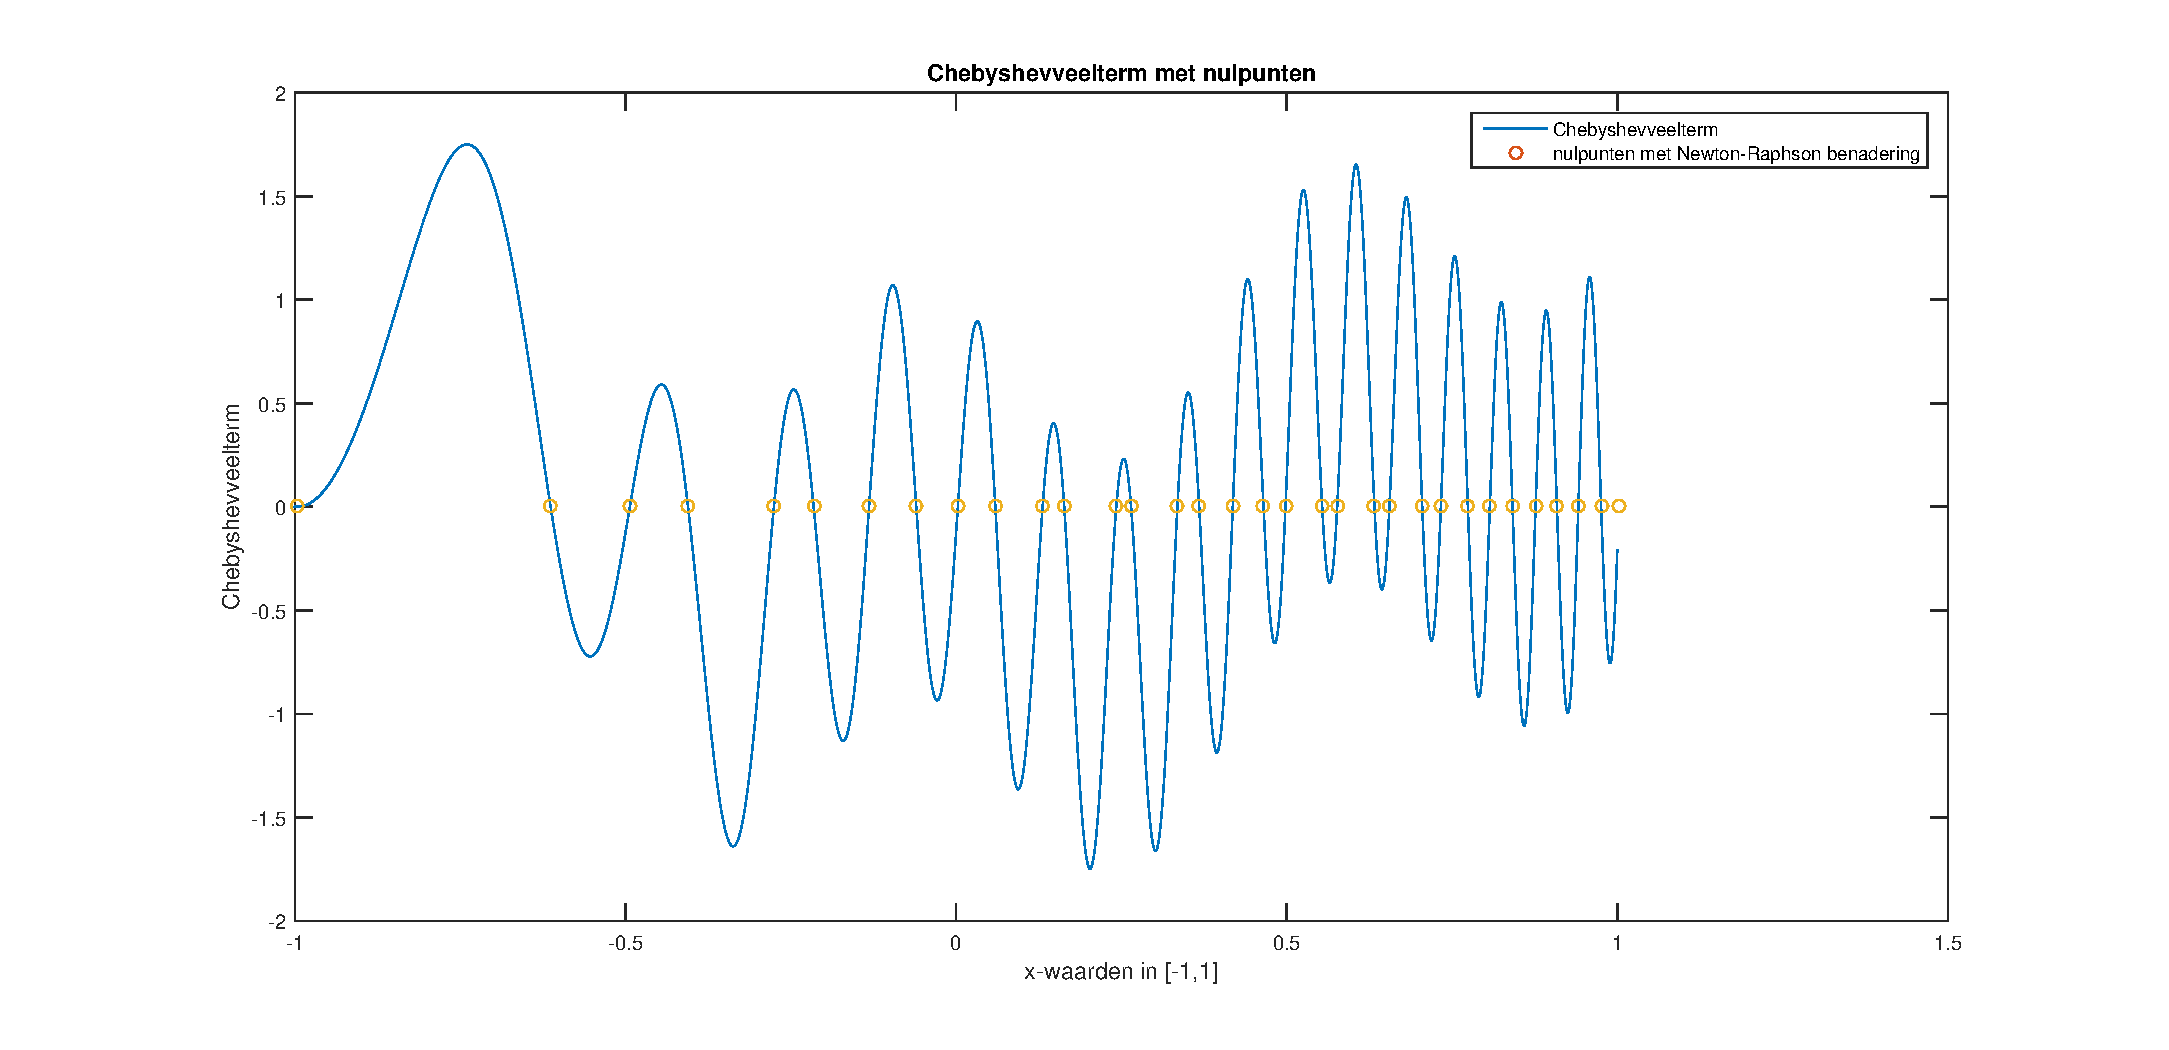
\includegraphics[width=0.60\columnwidth]{figuur_1}
\caption{Nulpuntbenadering met de methode van Newton-Raphson} % Example image
\end{figure}

Figuur 6 toont de veelterm die bekomen wordt door de vector c uit te zetten in de \textbf{Chebyshev basis}. Daarnaast worden ook de \textbf{nulpunten} weergegeven die gevonden worden m.b.v. de methode van Newton-Raphson. Het is duidelijk te zien dat alle nulpunten van de veelterm gevonden worden. Daarnaast worden er echter nog een aantal extra nulpunten berrekend die niet meer tot de veelterm behoren.
\\ \\
Om te zien welke startwaarde naar welk nulpunt convergeert, worden op onderstaande figuur de \textbf{residu\'\ s in functie van de startwaarden} geplot. De residu is de functiewaarde die bekomen wordt in de uiteindelijke benadering.
\\ \\

\begin{figure}[H]
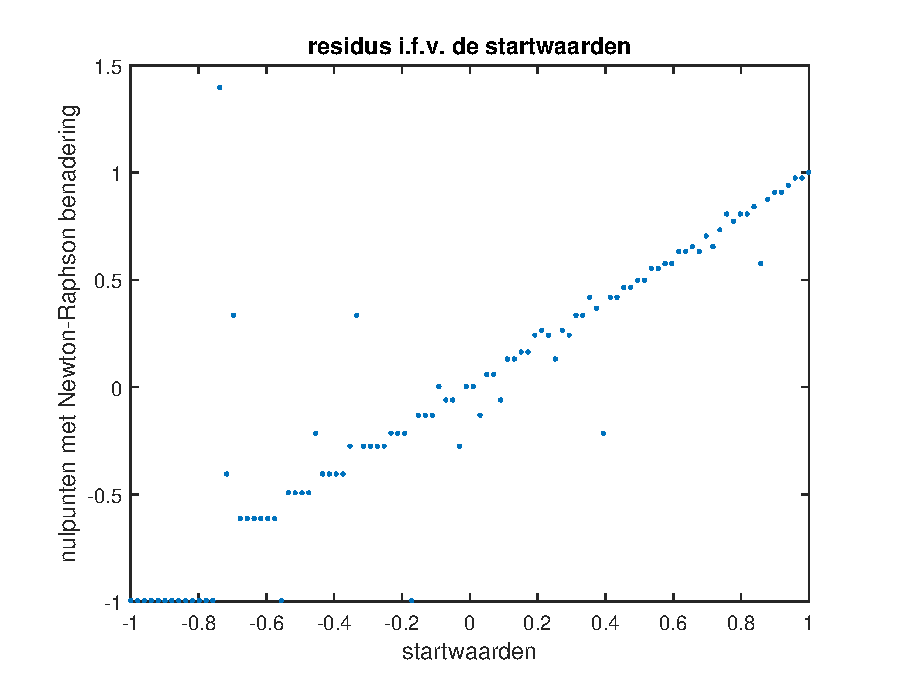
\includegraphics[width=0.75\columnwidth]{figuur_2}
\caption{Het residu in functie van de startwaarden $x_0$ = 0.9 en $x_0$ = 0.5} % Example image
\end{figure}

Het is makkelijk in te zien dat er \textbf{niet voor elk punt convergentie} zal zijn. De methode van Newton-Rapshon bepaalt immers een rij van punten waarvoor geldt: $x_{n+1}=x_{n}-\dfrac{f(x_{n})}{f’(x_{n})}$. Als ergens in deze rij $f’(x_{n})=0$ dan zal $x_{n+1}$ niet bestaan en is er dus geen convergentie. Een andere manier om de formule van Newton-Raphson te interpreteren is door $x_{n+1}$ te zien als het snijpunt van de x-as met de rechte door het punt $(x_{n},f(x_{n})$ in de richting van $f’(x_{n})$. Als $f’(x_{n})=0$ dan is deze rechte evenwijdig met de x-as, en er zal dus nooit een snijpunt zijn en dus ook geen convergentie.

\clearpage
\subsection{Fout en orde van convergentie voor verschillende startwaarden}
\ \\
\begin{figure}[H]
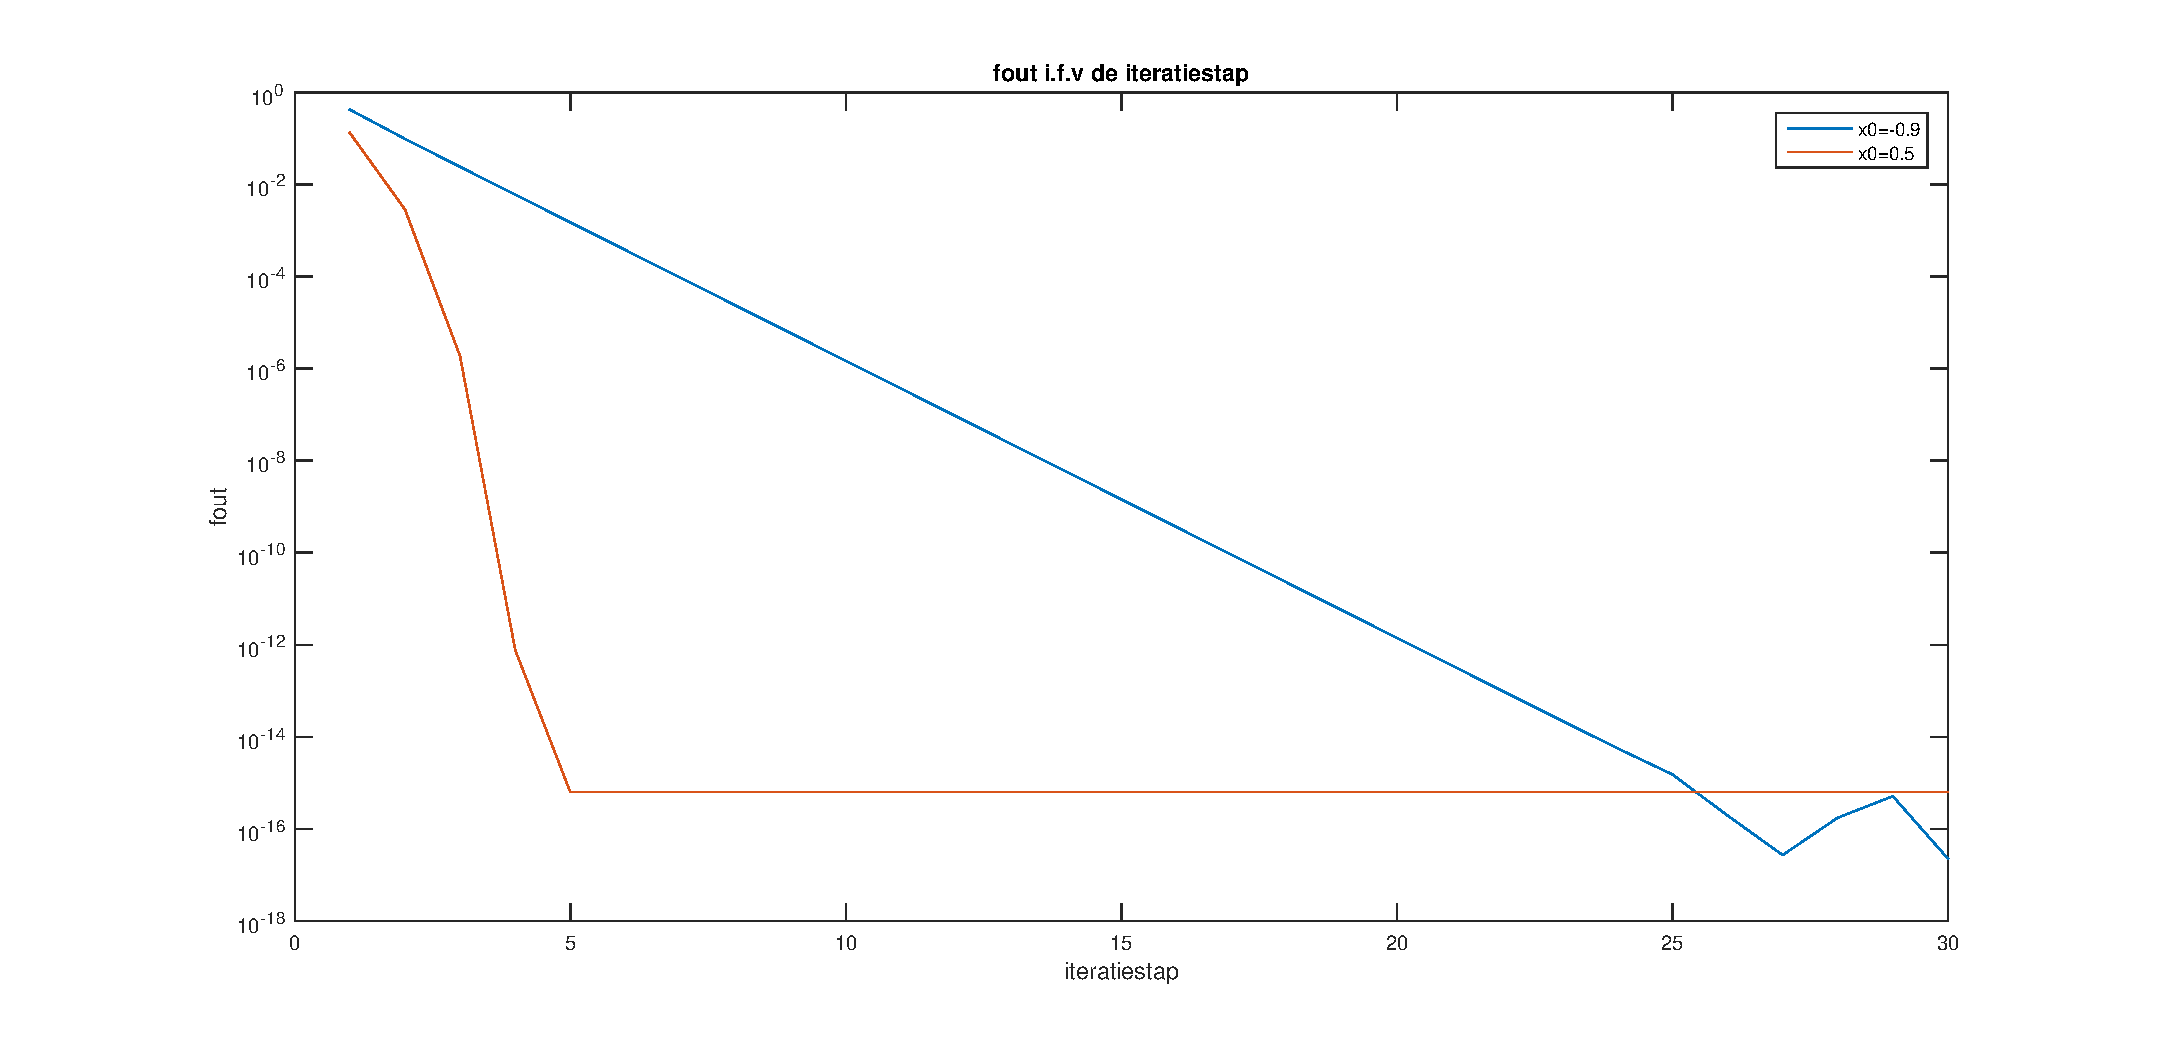
\includegraphics[width=0.75\columnwidth]{figuur_3}
\caption{Fout in functie van de iteratiesstap} % Example image
\end{figure}

Op figuur 7 is de fout in functie van de iteratiestap geplot voor de startwaarden $x_{0}=-0.9$ en $x_{0}=0.5$. Het is duidelijk merkbaar dat er voor de startwaarde 0.5 een veel snellere convergentie is. Met behulp van de formule $\rho_{p}=\lim_{n \rightarrow \inf } \dfrac{x_{n+1}-x{*}}{x_{n}-x{*}}$ kan de convergentie-orde bepaalt worden. Als $\rho_{p} $ een reëel getal is dan is n de orde van convergentie. Omdat er in de methode van Newton-Raphson maar een eindig aantal iteraties gebeurd, kan de limiet van n naar oneindig niet genomen worden maar moet het aantal iteraties in rekening gebracht worden. Het aantal iteraties hangt af van de nmax,het maximaal aantal iteraties, en de gekozen tolerantie, dit is het minimale verschil tussen twee opeenvolgende iteratiepunten. \\
Door toepassing van deze formule wordt voor de startwaarde -0.9 een convergentie-orde van 1 gevonden, deze convergeert dus lineair. Voor de startwaarde 0.5 is de convergentie-orde 2 en dus is er kwadratische convergentie.

\clearpage
\subsection{Fout en orde van convergentie met voorwaartse differenties}
\ \\
\begin{figure}[H]
\includegraphics[width=0.75\columnwidth]{figuur_4}
\caption{Fout in functie van de iteratiesstap} % Example image
\end{figure}

Vanaf nu wordt gebruikt gemaakt van de methode van Newton-Raphson waarbij de afgeleide berekend wordt m.b.v. voorwaartse differenties. Op Figuur 8 wordt de fout geplot voor startwaarde $x_{0}=0.5$ met verschillende waarden voor de parameter h. Op de figuur is duidelijk dat er \textbf{geen convergentie} is voor $h=10^{-1}$. Daarnaast lijkt het ook alsof er geen convergentie is voor $h=10^{-1.5}$ maar als de nmax verhoogt wordt tot 1000 dan is er toch convergentie merkbaar, de \textbf{convergentie-orde is wel zeer klein, ongeveer 0.05}.  Voor de andere waarden is er wel duidelijk convergentie dus kan de orde bepaald worden. Dit kan opnieuw met behulp van de formule die in de vorige paragraaf gegeven werd. Voor $h=10^{-2}$ is er \textbf{lineaire convergentie}. Voor $h=10^{-3}$ en $h=10^{-6}$ is er \textbf{kwadratische convergentie}.

\subsection{Extra rekenkost}
Stel dat de methode van Newton-Rapshon wordt toegepast, maar in plaats van de afgeleide te berekenen met behulp van voorwaartse differenties, worden nu centrale differenties gebruikt, dan is er \textbf{geen extra rekenkost}. Om een centrale differentie van orde n uit te rekenen moeten n+1 functie-evaluaties uitgevoerd worden. Dit is precies even veel als bij een voorwaartse differentie. \\
Het kan natuurlijk ook nog zijn dat een van de twee minder nauwkeurig is, en dat er dus meer differenties moeten gezocht worden om een afgeleide met een zelfde nauwkeurigheid te benaderen. Maar na evalueren van de formules van Gauss en Stirling, blijkt dat beide ongeveer even nauwkeurig zijn.




\clearpage

%----------------------------------------------------------------------------------------
\end{document}